\section{\sysname{} Overview}
\label{sec:system-overview}

In this section, we present an overview of \sysname{}. The primary goal of
\sysname{} is to enable applications with the ability to adapt its communication
in a guided manner.

\subsection{Challenges}
\label{sec:challenges}

\noindent There are four challenges in realizing \sysname{}.

\para{C1: Diverse application and data:} As discussed in~\autoref{sec:bat}, the
best adaptation scheme is often application- and context-specific
optimizations. It becomes important to separate individual application logic
from specific degradation strategy as well as adaptation mechanism.

\para{C2: No analytical solutions:} Unlike SQL queries whose demand and accuracy
can typically be estimated using analytical models~\cite{cormode2012synopses},
many of our streaming applications are dealing with unstructure data using
either use blackbox operations (such as H.264 encoding) or non-linear operators
(such as thresholding). The impact of these degradations is not immediately
available.

\para{C3: Multi-dimensional exploration:} Real-world applications typically have
more than one tunable parameters; leading to a combinatorial space for
exploration. In addition, these parameters are not necessarily orthognal.  The
optimal degradation strategies may only be achievable when more than one
degradation is in effect.

\para{C4: Runtime adaptation at application layer:} Although recent work on
resource reservation makes it possible to guarantee quality of service with new
IP or MAC layer protocols in LAN (e.g. TSN~\cite{johas2013heterogeneous}), we
target at WAN analytics where most of the infrastructure is owned by others and
shared among many users. An application-layer solution is in favor to those that
require special hardware or software upgrade.

\subsection{System Architecture}
\label{sec:architecture}

\begin{figure*}
  \centering
  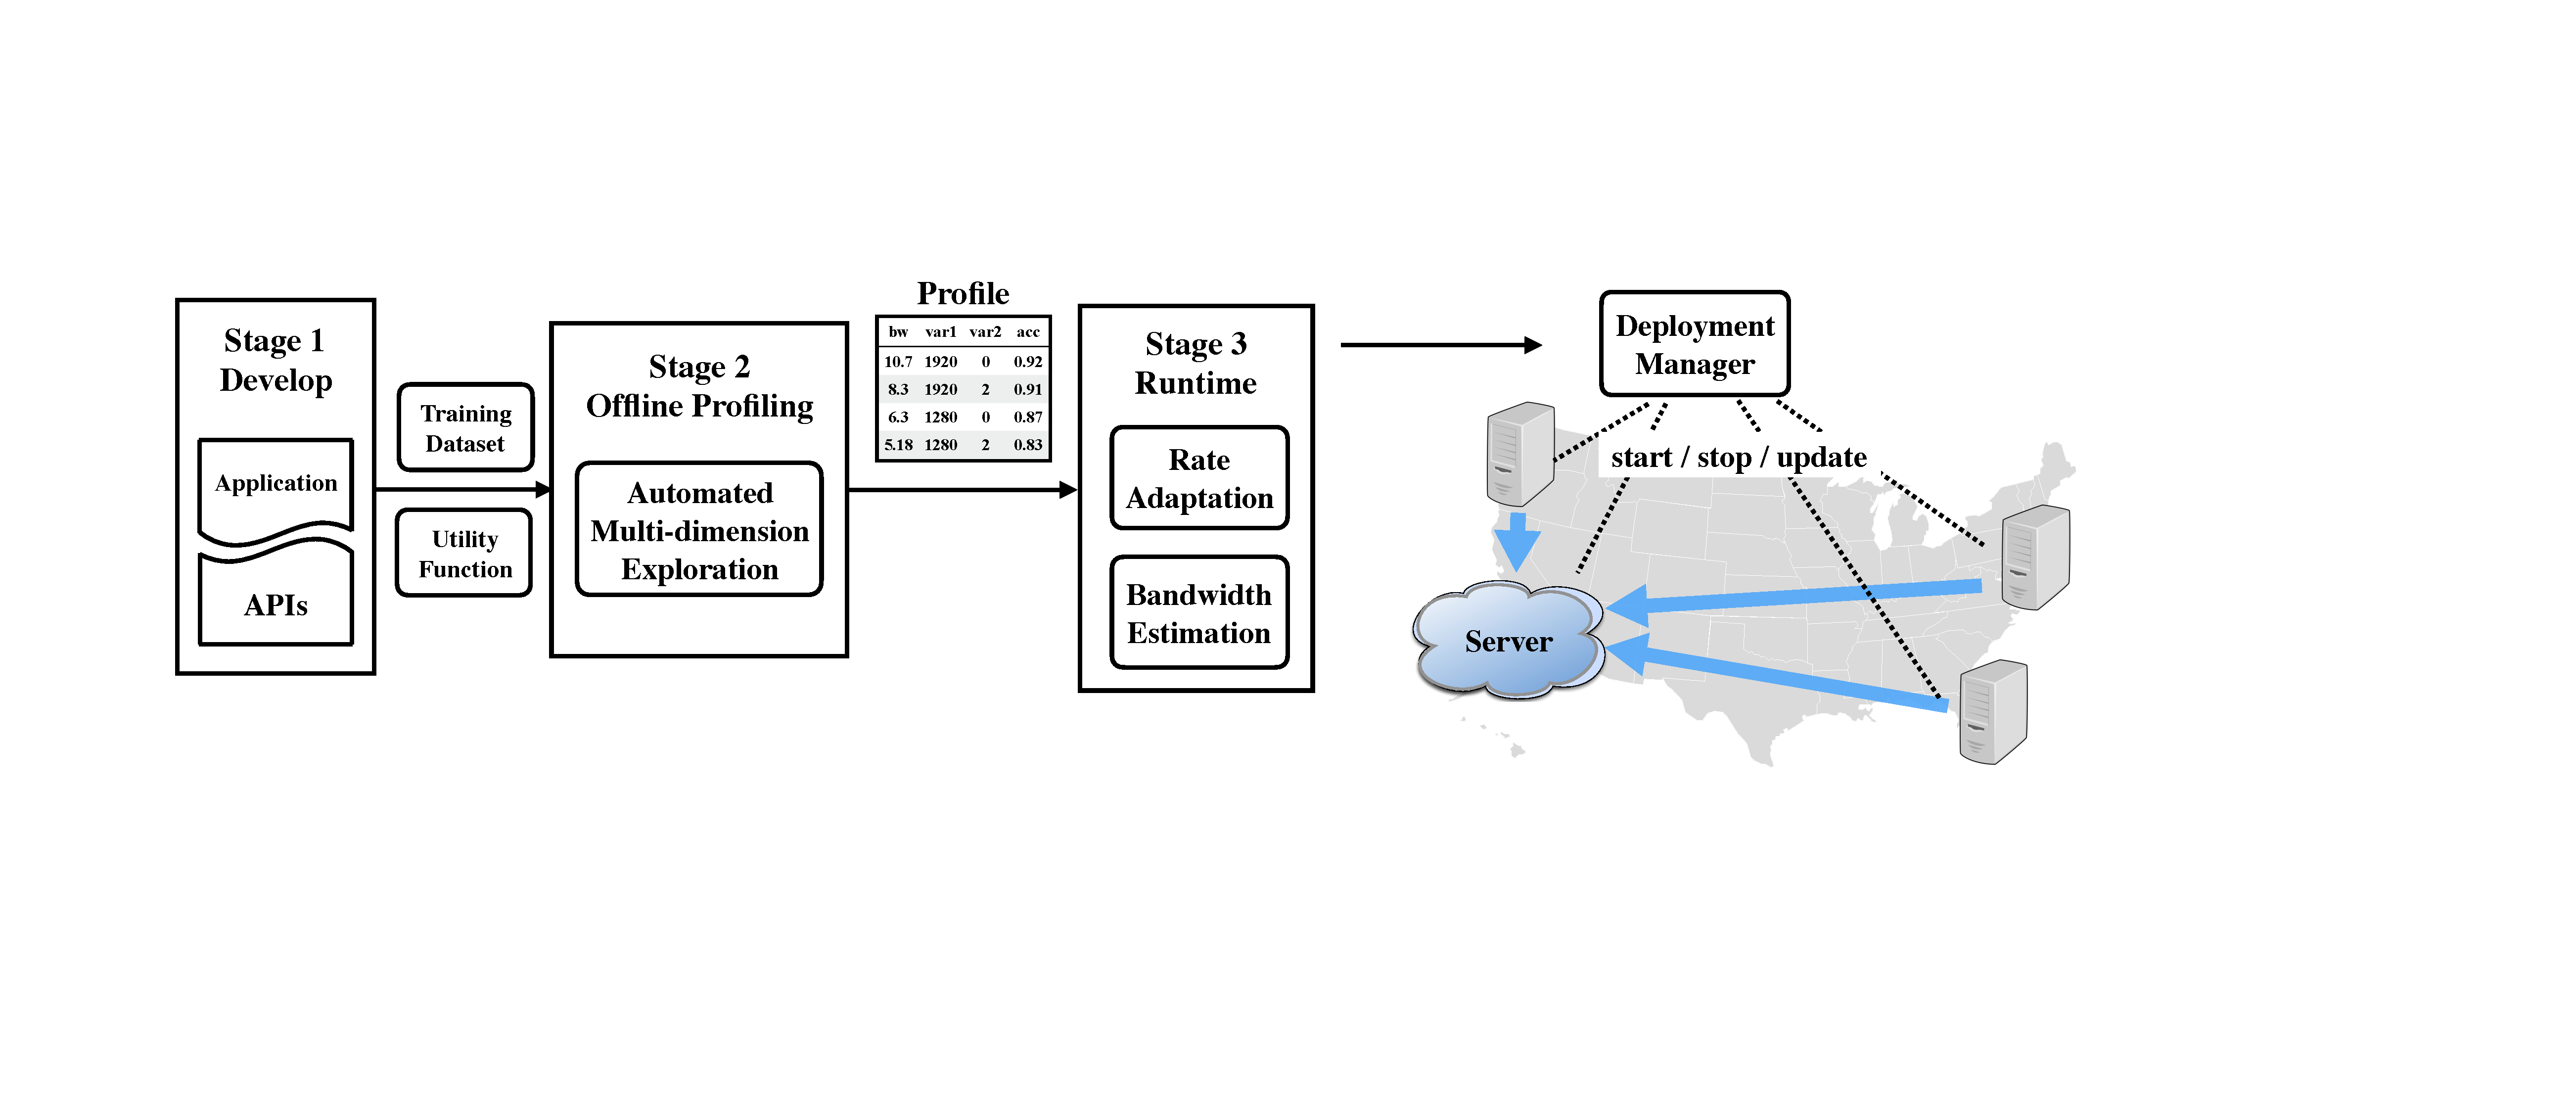
\includegraphics[width=\linewidth]{figures/arch.pdf}
  \caption{\sysname{} Overview.}
  \label{fig:overview}
\end{figure*}

To address the aforementioned challenges, \sysname{}'s solution is split into
four parts (\autoref{fig:overview}).

\para{Programming abstraction:} Applications are modelled as a directed acyclic
graph (DAG) of computation and we propose a novel set of \texttt{maybe}
operators to express the specification of degradation. Our propose APIs do not
require developers to be exact on the quantity; integrating this into existing
applications requires minimal effort (\autoref{sec:prog-abs}).

\para{Automatic multi-dimensional profiling:} Our system automatically explores
the parameter space to generate a Pareto-optimal degradation strategy with a
multi-dimensional exploration. We also report our experience and findings about
degradation operations (\autoref{sec:profiling}).

\para{Runtime Adaptation:} Finally the streaming application is deployed with a
wide-area orchestration manager. At runtime, our system generates additional
modules that acts as the control plane to adapt the application execution. The
control plane performs bandwidth estimation, congestion monitoring and
adaptation. It uses the profile generated from the second stage and adjust the
level of degradation (\autoref{sec:adaptation}).

%%% Local Variables:
%%% mode: latex
%%% TeX-master: "sigcomm2017"
%%% End:
